%
%	Begrifflichkeiten
%

\pagebreak
\section{TLS \& mTLS}

\onehalfspacing

\subsection{First}

\subsection{Rancher}

To easily manage the software installation on a Kubernetes cluster, we can turn to Rancher.

What is Rancher? The Rancher Labs website states it is "[...] a complete software stack for teams adopting containers. It addresses the operational and security challenges of managing multiple Kubernetes clusters while providing DevOps teams with integrated tools for running containerized workloads."\footnote{\textit{Rancher Labs (2025)}: Enterprise Kubernetes Management. \cite{rancher}}

Using a user-friendly GUI, Rancher provides a management platform for centrally managing multiple Kubernetes clusters in Enterprise IT. It also offers application development integration tools and robust enterprise-grade security and governance features. For operations, Rancher provides integrated solutions for logging, monitoring, and auditing, as well as many other features, such as CIS scans or a built-in service mesh.

The classic Rancher GUI looks like this:

\begin{figure}[H]
\centering
\caption {Rancher Dashboard}
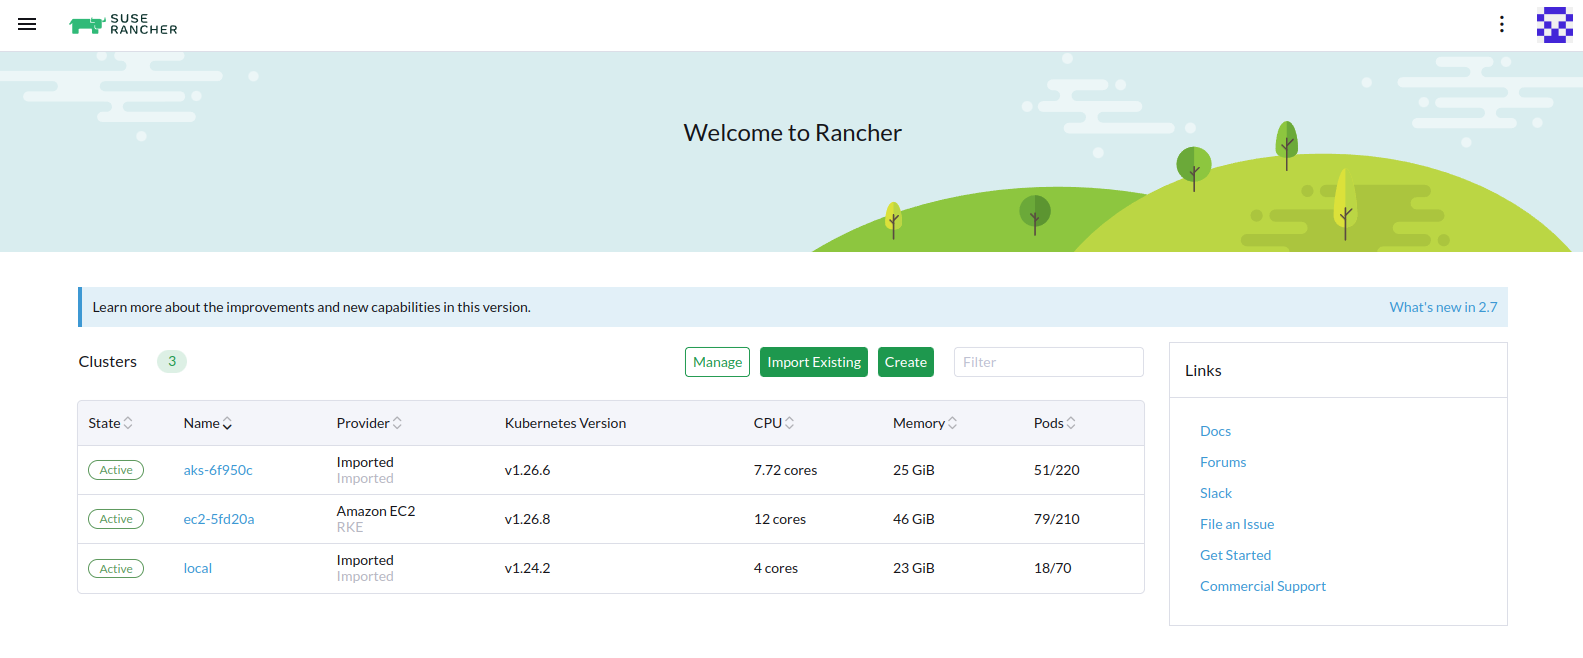
\includegraphics[width=\linewidth]{images/rancher-dashboard.png}
\label{fig:rancherDashboard}
\end{figure}

\subsection{Service Mesh}

Service Meshes is one of the cluster management applications available at Rancher.

Rancher includes installing the LInkerD and Istio applications for the various supported versions of downstream Kubernetes clusters.

Service Meshes can be installed within the Rancher UI as a Cluster Management application or using Infrastructure-as-Code automation, e.g., \href{https://www.terraform.io/}{Terraform}.
